

\documentclass[25pt,a0paper, portrait]{tikzposter}
\usepackage[utf8]{inputenc}
\usepackage{xcolor}
\usepackage{graphicx,mwe}
\usepackage{filecontents}
\usepackage{lipsum}
\usepackage{tikz}
\usepackage{multicol}
\usepackage{adjustbox}
\usepackage{blindtext}
\usepackage{comment}


\makeatletter
\def\TP@titlegraphictotitledistance{-5cm}
\settitle{ \centering \vbox{
		\@titlegraphic \\ [\TP@titlegraphictotitledistance] 
		\centering
		\color{titlefgcolor} 
		{\bfseries \Huge \sc \@title \par}
		\vspace*{1em}
		{\huge \@author \par}
}}
\makeatother

\setlength{\columnsep}{2cm}

\title{Counter Detection with ESP32}
\author{Alpizar, JK, \& Kumari}
\titlegraphic{
\includegraphics[height=6.5cm]{images/logo_hs_technik}
	\hfill
	
\includegraphics[height=6.5cm]{images/bida}
}


\usetheme{Desert}

\begin{document}
	
	
	\maketitle
	
	\begin{columns} 
		
		\column{0.36}
		{
			\colorlet{blocktitlebgcolor}{blue}
			\block{ESP32 microcontroller}
			{
				\begin{tikzfigure}
					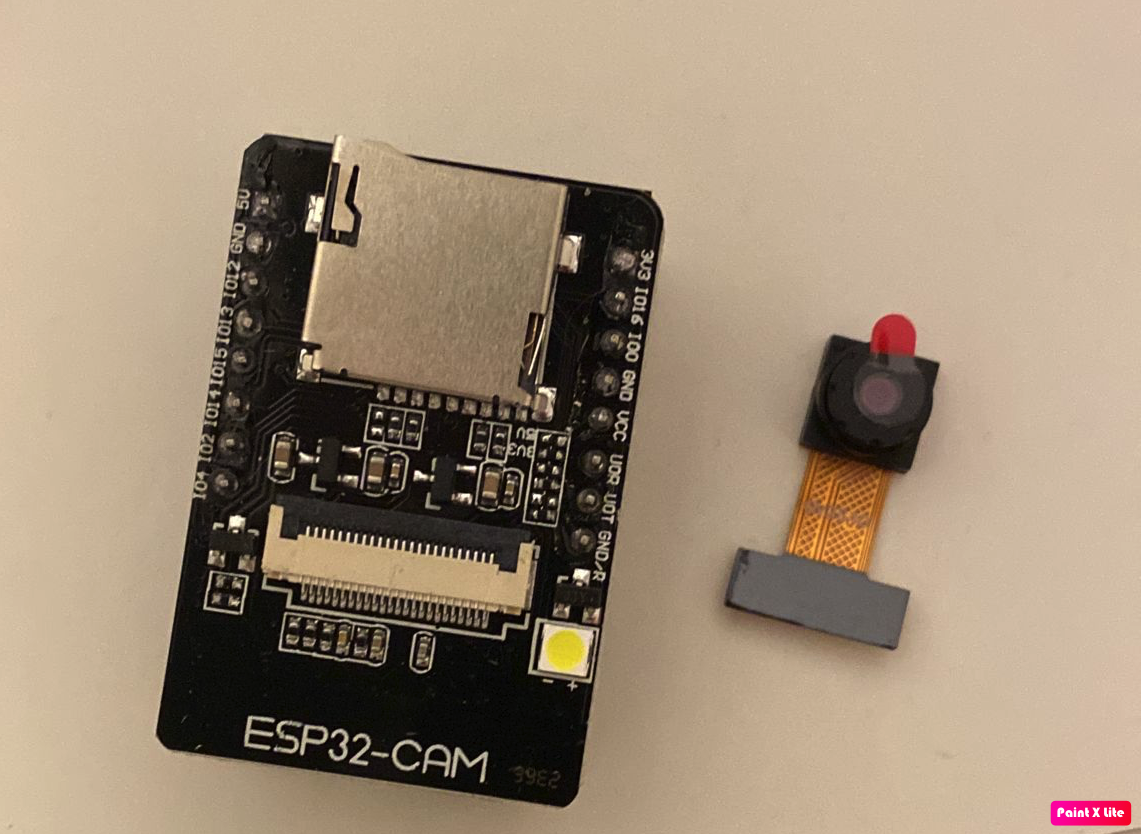
\includegraphics[width=\linewidth]{images/ESP32}
				\end{tikzfigure}	
			}
			\block{Problem description}
			{
				The goal of this project includes digitizing an analog meter. Initially, by recognizing one digit using ESP32-CAM and TFLite libraries with the help of a model trained using Convolutional Neural Network (CNN) algorithm. This would be useful in monitoring energy usage or measuring the output of a device.
			}
		}
		
		
		\column{0.64}
		{
			\colorlet{blocktitlebgcolor}{blue}
			\block{Trained model}
			{
				\begin{tikzfigure}
					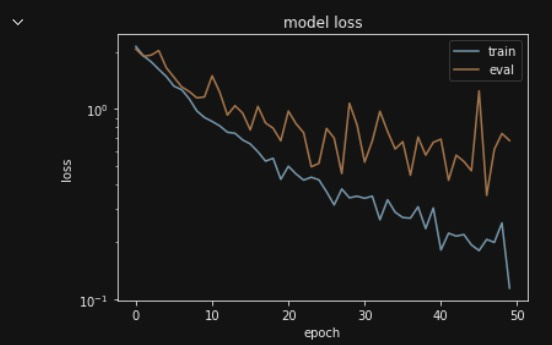
\includegraphics[width=\linewidth]{images/TrainedModel}
				\end{tikzfigure}	
			}
				
			}
	\end{columns}
	
	\begin{columns} 
		
		\column{0.60}
		{
			\colorlet{blocktitlebgcolor}{blue}
			\block{Confusion Matrix }
			{
				\begin{tikzfigure}
					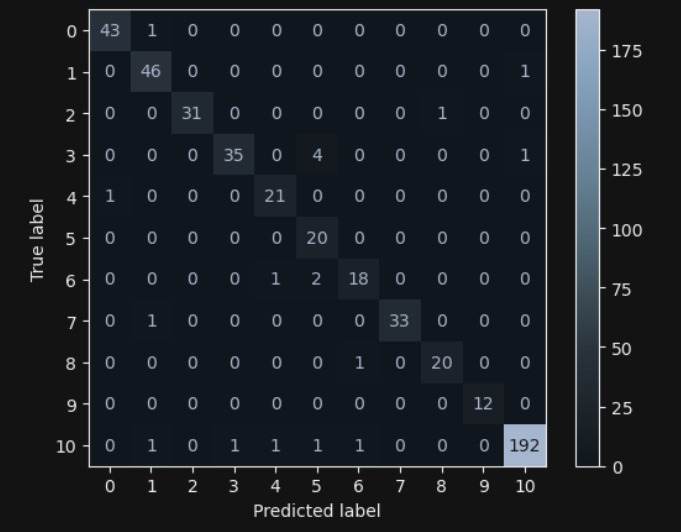
\includegraphics[width=\linewidth,keepaspectratio]{images/ConfusionMatrix}
				\end{tikzfigure}
				
			}
			\block{Water meter}
			{
				\begin{tikzfigure}
					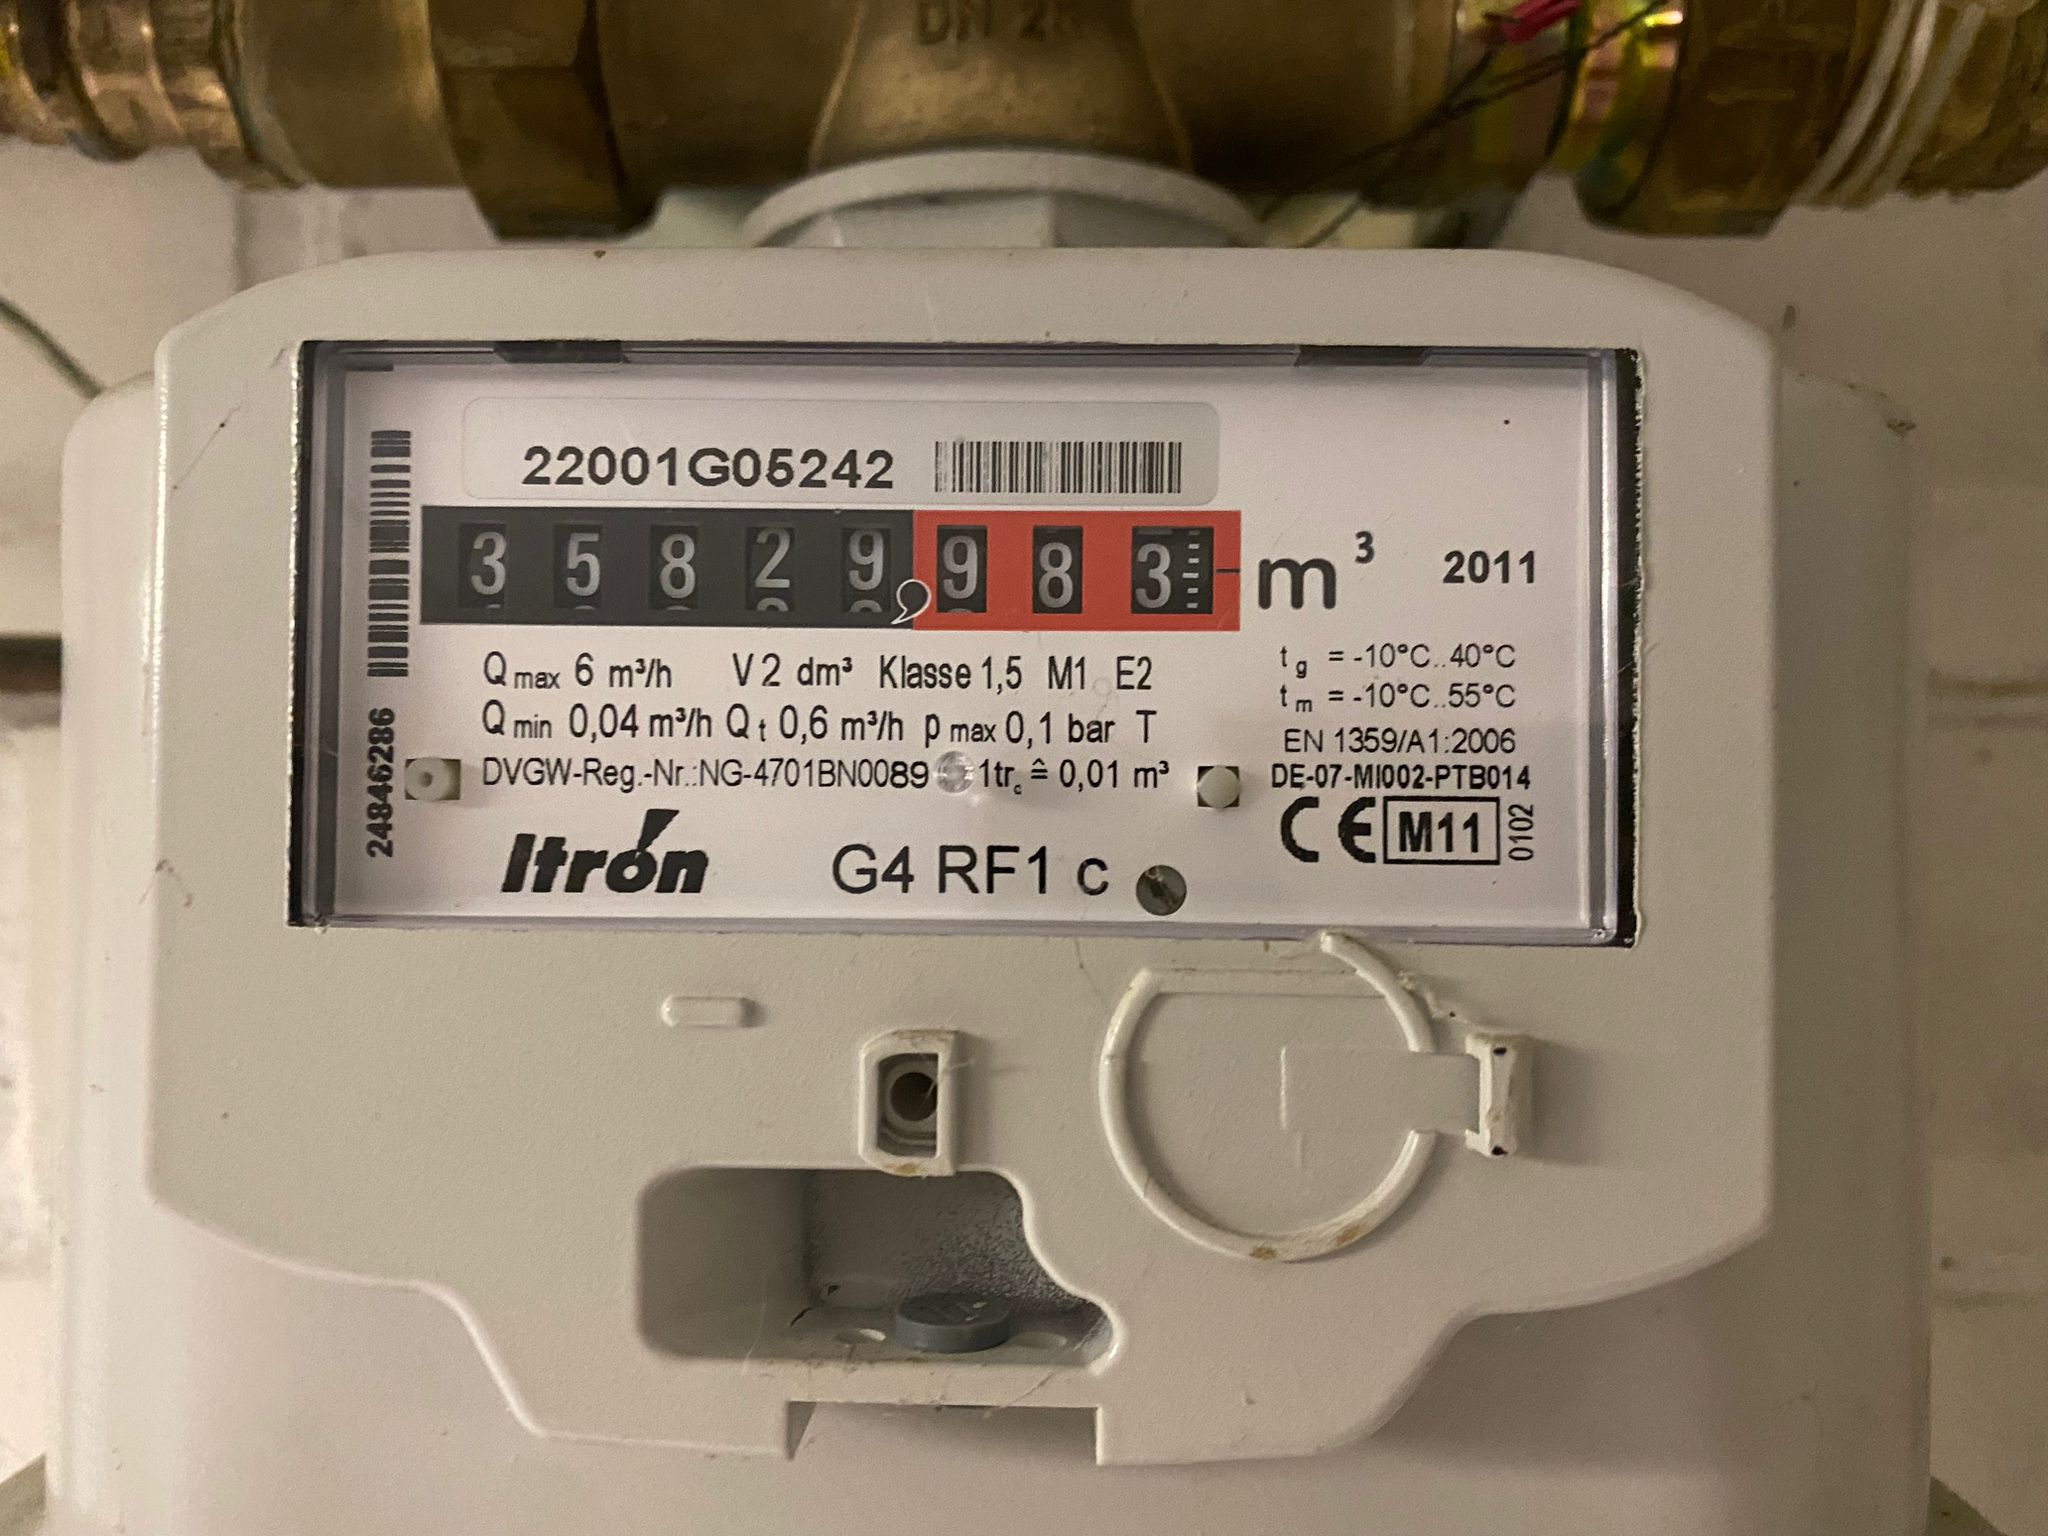
\includegraphics[width=20cm]{images/watermeter}
				\end{tikzfigure}	
			}
		}
		
		
		\column{0.40}
		{
			\colorlet{blocktitlebgcolor}{blue}
			\block{Implementation and Challenges}
			{
				This project includes use of TinyML model on an ESP32 microcontroller to digitize an analog meter. The model is trained using CNN algorithm.\\
				A CNN is a type of artificial neural network specifically designed to process data with a grid-like topology, such as an image. CNNs are preferred for image classification tasks because they are able to automatically learn and extract features from the input data, which makes them well-suited to tasks where the features of interest may not be easily defined by humans. The steps include preprocessing, convolutional layers, pooling and classification.\\
				
				Certain challenges are that ESP32 used for image processing in ML might be short on resources and storage. Also, data Labelling and Collection ( multiple analog meters) is a time consuming activity. Although, ESP32 is well-suited for this task due to its low power consumption and powerful processing capabilities but running ML models can still consume a lot of power. Need to consider appropriate power source.
			}
			\block{Future Improvements}
			{
				\begin{itemize}
					\item Implement a mobile application with user settings and specific account management.
					\item A Log-In module that can track users actions in the application, and responses from the counter
					\item A more robust HW implementation where the counter detection can be located easily in front of the meter. 6.1
					\item Develop a more complex CNN using a more powerful development tool like OpenCV and Raspberry Pi as platform, to have more processing capabilities.
				\end{itemize}
			}
		\block{Digit recognition}
		{
			\begin{tikzfigure}
				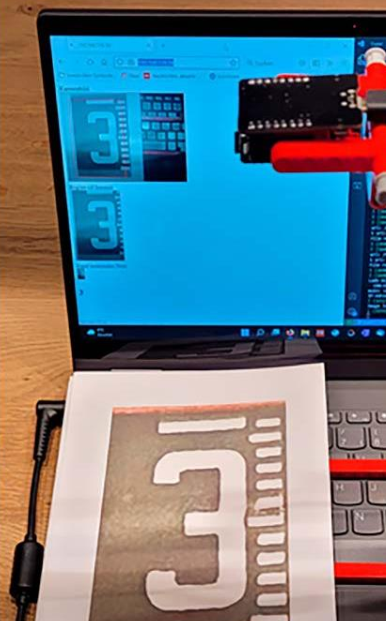
\includegraphics[width=8cm]{images/ESP32CAM_Field}
			\end{tikzfigure}	
		}
		}
	\end{columns}
	
\end{document}

